\chapter{Part pràctica}
\label{c:Partpra}

L’objectiu dels experiments realitzats en aquesta part pràctica és avaluar la qualitat de l’aigua mitjançant l’ús de tires reactives. Per fer-ho, es van dur a terme tres experiments concrets, dissenyats per analitzar diversos paràmetres clau de l’aigua.

A més de presentar els resultats obtinguts, aquesta recerca també proporciona una sèrie de recomanacions sobre com utilitzar les tires de manera correcta, amb l’objectiu d’obtenir mesures més fiables i precises.


\section{Primer experiment}

% Vaig començar a organitzar-me i a buscar el material que hauria d’utilitzar per fer la part pràctica. La meva intenció era llegir una mica i complir un dels objectius que m’havia proposat per a l’estiu. No acostumo a llegir gaire; per això, si llegir per informar-me m’ajudava, ho feia amb molt de gust. Amb l’ajuda del meu tutor, Fernando, vaig trobar unes tires reactives a Amazon que em permetrien analitzar químicament l’aigua. Amb una sola tira es poden mesurar fins a setze paràmetres diferents. Aquestes tires tenien un cost de 19,99 euros. També disposava d’un mesurador digital de pH, cedit per l’institut, que considerava el material més fiable, ja que proporciona una lectura exacta i no un valor aproximat.

Tal i com es fa qualsevol experiment científic, la primera part d'un experiment consisteix en el disseny i l'obtenció del material. El material necessari per elaborar l'experiment es troba al capítol \ref{c:Metodologia}~\nameref{c:Metodologia}, a la secció~\ref{s:recursos}.

% L’objectiu principal era determinar la concentració de diferents compostos en una mostra d’aigua concreta i comparar-ne els resultats amb les dades oficials disponibles. Abans de fer la comparació, primer necessitava extreure les meves pròpies dades. Gràcies al material que tenia, podia obtenir resultats per més d’una via i comparar entre si les dades obtingudes i les oficials. La raó de fer-ho de diverses maneres era avaluar quina era la més eficient i, si era possible, posar a prova la fiabilitat de les dades oficials mitjançant l’experimentació directa.

%%%% Simplement actualitzo el temps verbal. Hauries de fer el mateix a la resta del treball
L’objectiu principal de l'experiment és determinar la concentració de diferents compostos en una mostra d’aigua concreta i comparar-ne els resultats amb les dades oficials disponibles. Abans de fer la comparació, primer necessitava extreure les meves pròpies dades. Gràcies al material del que disposo, puc obtenir resultats per més d’una via i comparar entre si les dades obtingudes i les oficials. La raó de fer-ho de diverses maneres és avaluar quina és la més eficient i, si és possible, posar a prova la fiabilitat de les dades oficials mitjançant l’experimentació directa.

Tan bon punt em van arribar les tires, vaig iniciar els experiments. La primera prova va consistir a recollir aigua de l’aixeta de casa meva. Vaig utilitzar una ampolla buida per emmagatzemar-la. El pas següent era entendre el funcionament de les tires que havia comprat. L’únic inconvenient era que el pH i el nitrit es repetia en els dos metodes, per això vaig decidir mesurar-lo per les tres vies: amb les tires reactives, amb el mesurador digital i amb el TetraTest de nitrit.

%Això als agraïments..., aquí no.
% Gràcies a les explicacions de l’Àlex Tuca, ara ja puc fer servir correctament el mesurador de pH. Segons les seves instruccions, un cop feta la mesura, cal netejar el dispositiu amb aigua destil·lada.

Abans de començar l'experiment, vaig haver d’investigar com utilitzar correctament les tires. Per fer-ho, vaig documentar-me alguns vídeos tutorials~\cite{VideosDeSuport} i consultar altres fonts~\cite{FontsPerTires}. El procediment correcte és submergir la tira durant un segon i retirar-la immediatament. En aquest punt va aparèixer un dubte: en alguns vídeos deixaven assecar la tira al sol i en altres no. Per tal de determinar si aquest fet era rellevant per als resultats, vaig decidir provar tots dos mètodes i comparar els resultats. Aquesta decisió va prendre més sentit quan vaig descobrir que a les instruccions l’envàs exterior (en anglès), s’indicava que les tires no havien de tenir contacte amb la llum solar directa, però, sorprenentment, a l’interior —també en anglès— les instruccions deien el contrari: que s’havien d’assecar al sol. Aquesta incoherència em va deixar clar que calia fer l’experiment de les dues maneres.

% La decisió de fer l'experiment amb i sense llum solar també apareixa com una contradicció en les instruccions del paquet. A l’envàs exterior (en anglès), s’indicava que les tires no havien de tenir contacte amb la llum solar directa. Però, sorprenentment, a l’interior —també en anglès— les instruccions deien el contrari: que s’havien d’assecar al sol. Aquesta incoherència em va portar a fer l’experiment de les dues maneres.

%%%%%%%%%%%%%%%%%%%%%%%%%%%%%%%%%%%%%%%%%%%%%%
%%%%%%%%%%%%%%%%%%%%%%%%%%%%%%%%%%%%%%%%%%%%%%

Un cop tot es material ja estava disponible, va començar l'experiment. Tots els passos realitzats i els resultats obtinguts han estat anotats en una llibreta dedicada especialment per a aquest projecte.

%%% Revisa els temps verbals -> encara cal fer-ho...
Abans de començar oficialment amb les mesures, organitzo totes les mostres. L’aigua de l’aixeta la guardo en una ampolla de plàstic degudament etiquetada per no confondre-la amb altres mostres. També col·loco etiquetes a gairebé tot: les tires, segons si s’assecaran amb o sense llum solar i els gots amb les diferents aigües.

\begin{figure}[h]
\centering
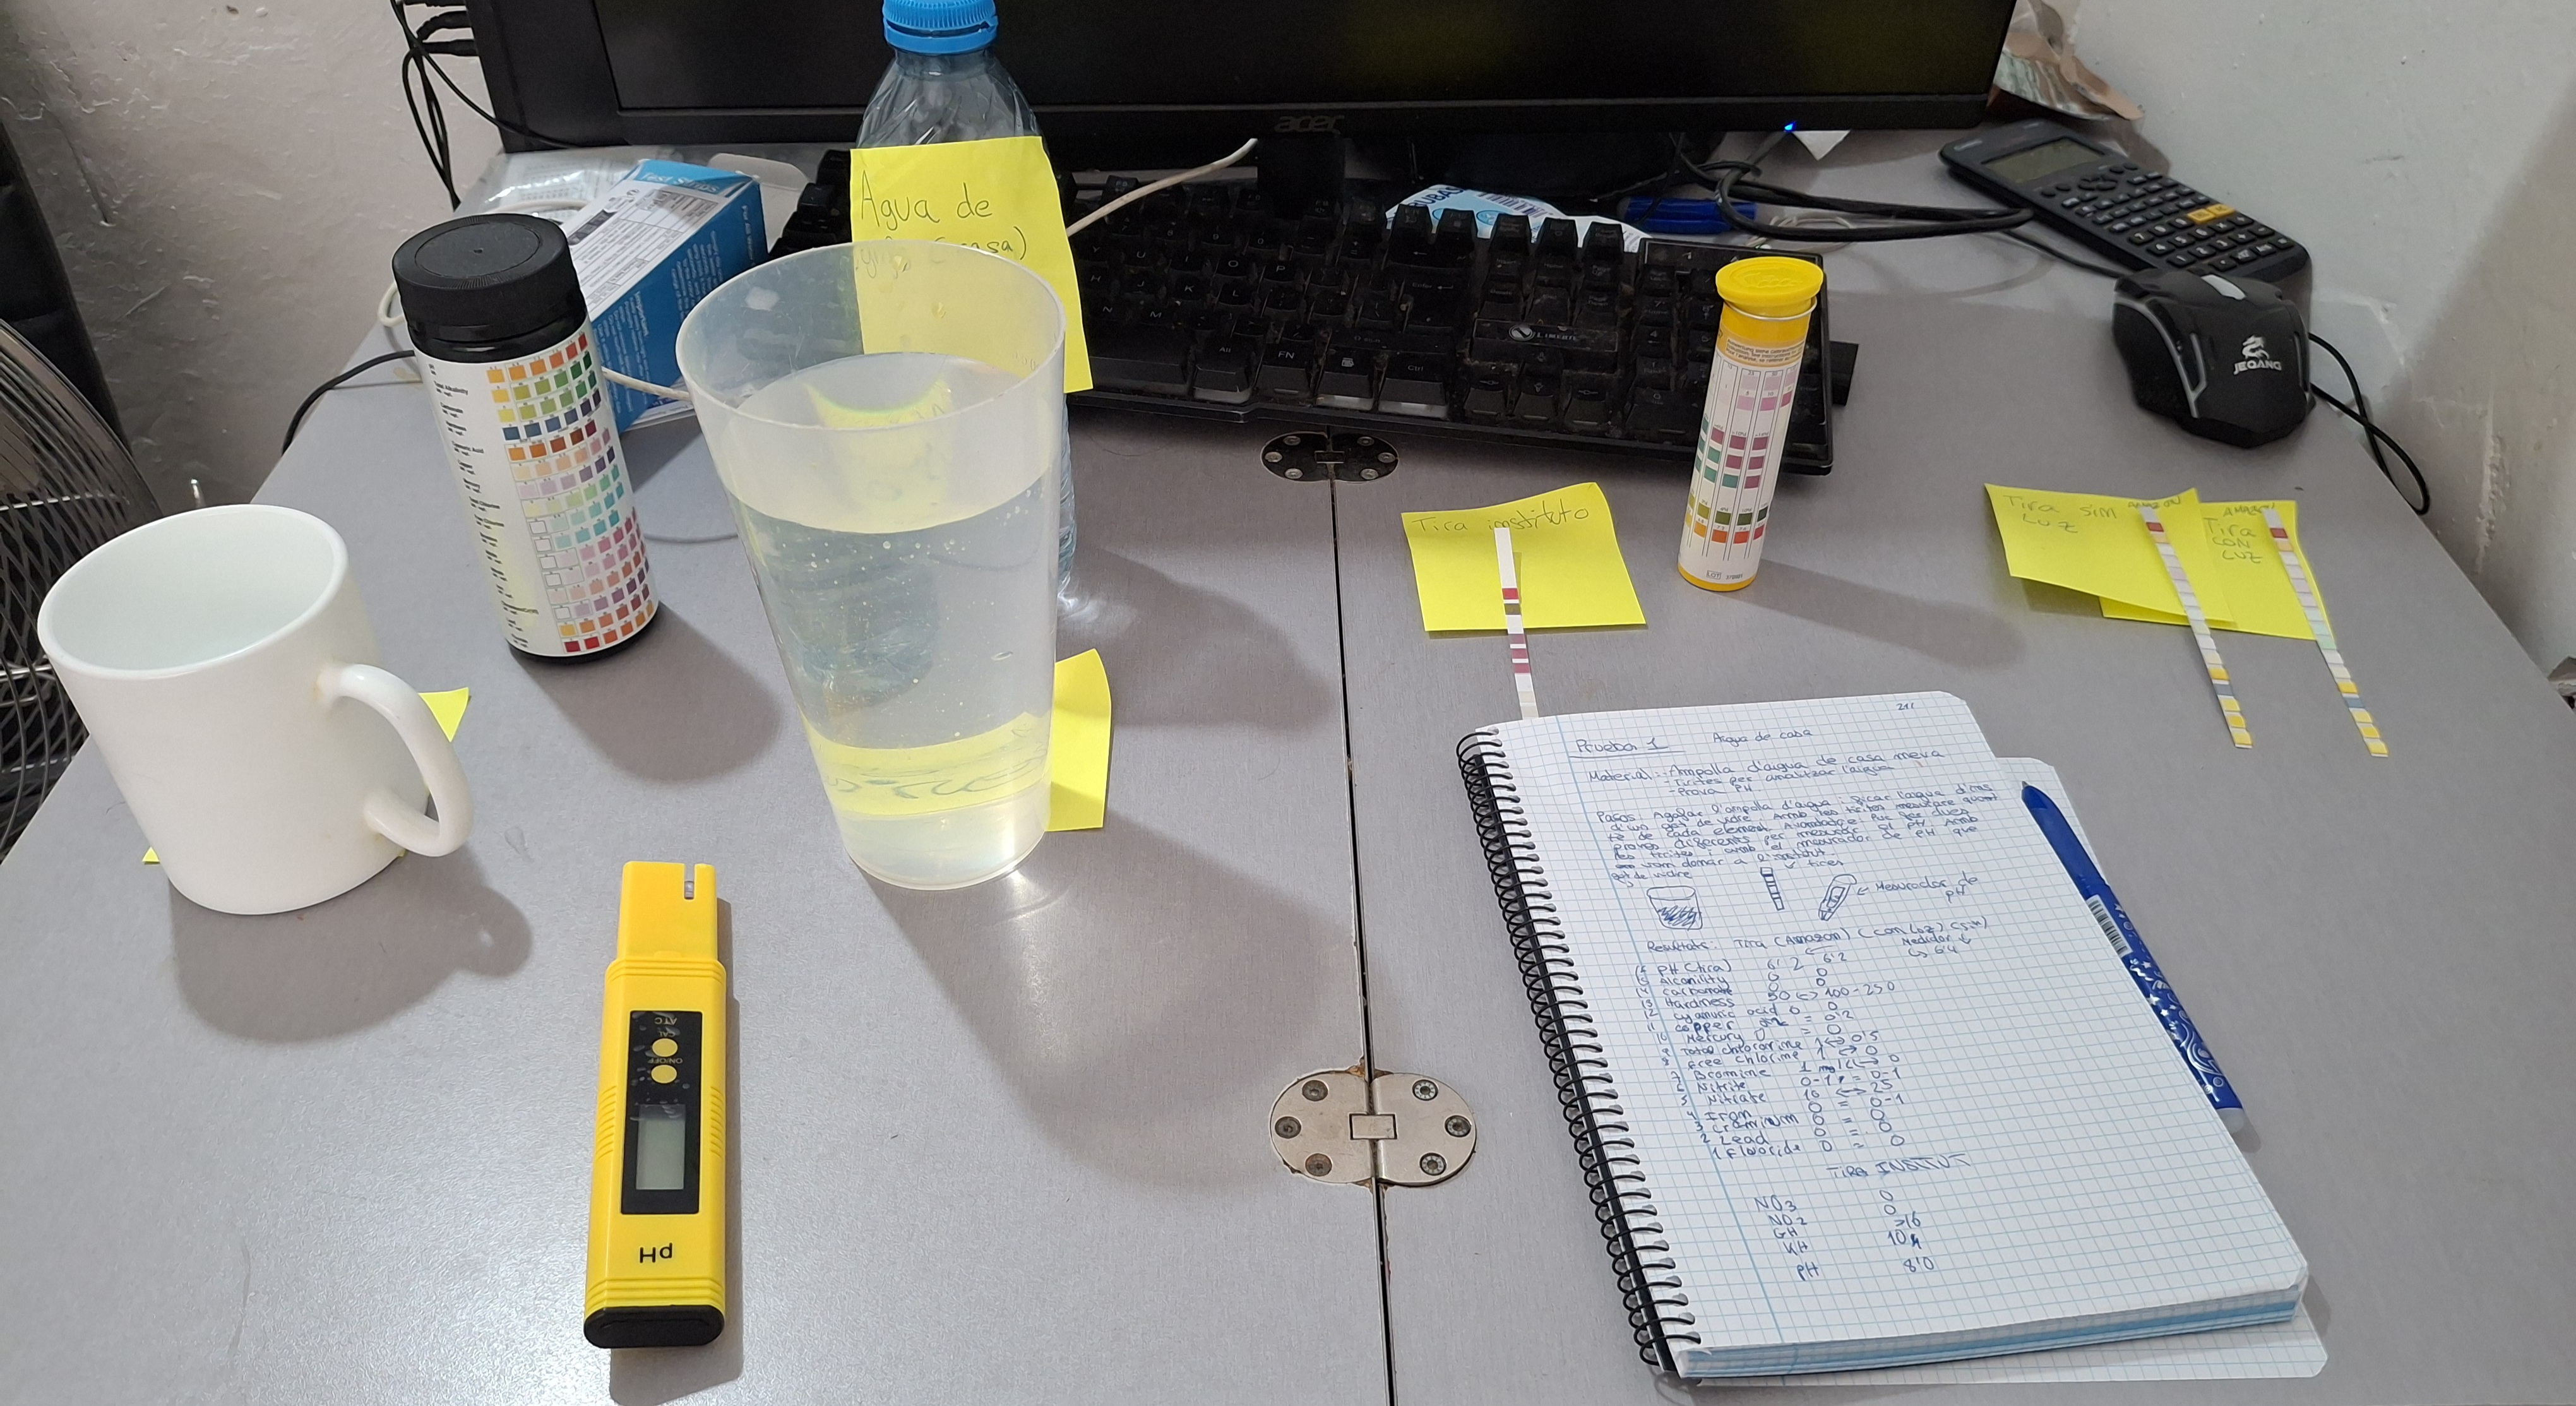
\includegraphics[width=0.9\textwidth, angle=0]{./Figures/expe.png}
\caption{Pre-experiment }
\label{fig:fotoPreExperiment}
\end{figure}

Els passos que vaig seguir van ser els següents: en un got hi vaig posar l’aigua de l’aixeta i en un altre, l’aigua destil·lada. Vaig començar utilitzant les tires d’Amazon, però em vaig adonar que els components químics estaven escrits en anglès, així que vaig haver-los de traduir per saber què estava mesurant i poder anotar-ho a la llibreta.

Després d’assecar la tira durant 60 segons, ja es podien observar els colors que indicaven la presència i concentració de cada compost. Segons la intensitat del color, es podia determinar el valor aproximat. Ara bé, aquest sistema presentava una dificultat: els colors no sempre eren clars ni fàcils de comparar amb la guia de referència, cosa que feia que els resultats fossin sempre aproximats i no totalment precisos.

Primer vaig fer la prova amb les tires exposades a la llum solar. A continuació, vaig repetir l’experiment amb una tira nova, però aquesta vegada sense exposició solar.
% Es mostren els resultats obtinguts al \textit{Appendix}~\ref{s:A1}, a la taula \ref{tab:comparacio_dades}~\nameref{tab:comparacio_dades}.


Tal com es pot veure a la taula~\ref{tab:comparacio_dades}, en general no hi ha diferències molt grans entre fer la prova amb o sense exposició solar. Tot i així, hi ha alguns casos destacats. Per exemple, la duresa presenta un salt important: 50 mg/L amb llum solar, i 175 mg/L sense. També els nitrats mostren una diferència significativa: 10 mg/L amb sol i 25 mg/L sense. Altres compostos com el ferro o el clor total mostren variacions més lleus, però també notables. En canvi, el clor lliure apareix amb 1 mg/L en la tira exposada al sol, i 0 mg/L en la que no hi ha estat.

\begin{table}[H]
\centering
\resizebox{\textwidth}{!}{
\begin{tabular}{|c|c|p{4.4cm}|}
\hline
\textbf{Paràmetre} & \textbf{Resultats amb llum solar en mg/L} & \textbf{Resultats sense llum solar en mg/L} \\
\hline
pH    & 6.2      & 6.2 \\
\hline
Alcalinitat total(CaCO$_3$)    & 0    & 0 \\
\hline
Carbonat     & 0      & 0 \\
\hline
Duresa (GH)   & 50          & 175  \\
\hline
Àcid cianúric    & 0     & 0 \\
\hline
Coure    & 0.2       & 0.1\\
\hline
Mercuri    & 0      & 0 \\
\hline
Clor total     & 1     & 0.5\\
\hline
 Clor lliure    & 1      & 0 \\
\hline
Brom  & 1      & 0\\
\hline
 Nitrit    & 0.5       & 0.5\\
\hline
Nitrat (NO$_3^-$)    & 10        & 25 \\
\hline
Ferro    & 0      & 0.5 \\
\hline
 Crom (VI)   & 0      & 0  \\
\hline
Plom   & 0     & 0  \\
\hline
Fluorur (F$^-$)    & 0      & 0 \\
\hline
\end{tabular}%
}
\caption{Resultats del primer experiment}
\label{tab:comparacio_dades}
\end{table}

\clearpage
Un cas especialment curiós ha estat el del pH, ja que els dos mètodes emprats han coincidit en un valor de 6.2 mg/L. Inicialment pensava que aquest seria un dels valors més variables.
%%% Aquí pots investigar per si trobes una explicació possible!!!

Una possible explicació d’aquesta estabilitat és que el pH de l’aigua no es veu afectat significativament per l’exposició solar. El pH depèn principalment de la concentració d’ions H$^+$ i OH$^-$, i aquestes concentracions romanen relativament estables si l’aigua no conté compostos fotosensibles. Com que l’aigua utilitzada no presenta una alcalinitat ni una presència de compostos reactius significativa, la llum solar no n’ha alterat el pH. Això suggereix que les condicions ambientals d’aquest experiment no afecten aquest paràmetre en concret.

Després de fer la prova amb les tires reactives, procedeixo a repetir-la amb el mesurador digital de pH. El resultat que obtinc és notablement diferent del que indiquen les tires: el valor mesurat és de 7.21 mg/L. Aquesta diferència posa en evidència la limitació de les tires reactives, que només permeten una estimació aproximada, mentre que el mesurador proporciona una dada precisa.

Les dades reals de l’aigua les vaig consultar a la web d’Aigües de Barcelona~\cite{qualitatAigua}. Un cop feta la comparació, aquests són els resultats obtinguts amb les dues tires, tant amb exposició solar~\ref{tab:comparacio_aigua_amb_sol} com sense~\ref{tab:comparacio_aigua_sense_sol}.
% Les taules es poden veure al \textit{Appendix}~\ref{s:A1}~ ~\nameref{tab:comparacio_aigua_amb_sol} i~\nameref{tab:comparacio_aigua_sense_sol}
Com es pot veure en les dues comparacions, les tires reactives han fallat en gairebé tots els casos pel que fa als valors obtinguts. Tot i això, la tira sense exposició solar ha mostrat resultats més propers als valors originals. Per tant, segons aquesta comparació, puc concloure que és millor no exposar la tira a la llum solar. A més, els valors que ens aporten són diferents, per tant, ens hem de limitar només als que coincideixen en ambdós casos.

També cal aclarir que hi ha determinats paràmetres que no es tenen en compte en l’aigua potable, i això fa que sigui impossible comparar-los. El que més m’ha sorprès, però, ha estat la comparació següent:

\begin{minipage}[h]{1\textwidth}
  \begin{table}[H]
  \centering
  %\resizebox{\textwidth}{!}
  \caption{Comparació entre els valors experimentals i els oficials de l'aigua de l'aixeta (amb el mesurador de pH)}
  \label{tab:comparacio_mesurador_ph1}
\end{table}
\end{minipage}
\clearpage

\begin{table}[H]
\centering
\resizebox{\textwidth}{!}{
\begin{tabular}{|l|c|c|c|p{4.4cm}|}
\hline
\textbf{Paràmetre} & \textbf{Valor experimental} & \textbf{Valor oficial} & \textbf{Unitats} & \textbf{Comentari} \\
\hline \hline
pH & 6,2 & 7.2-8.3 & unitats pH & Inferior al valor oficial; aigua més àcida. \\
\hline
Alcalinitat total & 0 & 158-210 & mg CaCO$_3$/L & Valor experimental probablement incorrecte. \\
\hline
Carbonats & 0 & --- & mg /L & Informació no proporcionada. \\
\hline
Duresa total & 50 & 222-309 & mg GH /L & Molt inferior al valor oficial. \\
\hline
Nitrat & 10 & 5.2-11.1 & mg NO$_3^-$ /L & Lleugerament superior; dins de marges acceptables. \\
\hline
Nitrit & 0.5 & ---& mg /L & Informació no proporcionada. \\
\hline
Clor total & 1 & --- & mg/L & Valor comú en aigües potables. \\
\hline
Clor lliure & 1 & --- & mg/L & Idèntic al valor anterior. \\
\hline
Ferro & 0 & --- & mg/L & No detectat; valor desitjable. \\
\hline
Fluorur & 0 & $<$0,2 & mg F$^-$ /L & Coincideix amb el límit inferior. \\
\hline
Crom (VI) & 0 & --- & mg/L & No present, tal com és recomanable. \\
\hline
Plom & 0 & --- & mg/L & Absent, com hauria de ser. \\
\hline
Àcid cianúric & 0 & --- & mg/L & No rellevant en aigua potable. \\
\hline
Coure & 0,2 & --- & mg/L & Informació no detectada en aquest cas. \\
\hline
Brom & 1 & --- & mg/L & No habitual en aigua potable. \\
\hline
Mercuri & 0 & --- & mg/L & No present; correcte. \\
\hline
\end{tabular}%
}
\caption{Comparació entre els valors experimentals i els oficial (amb exposició solar)}
\label{tab:comparacio_aigua_amb_sol}
\end{table}

\begin{table}[H]
\centering
\resizebox{\textwidth}{!}{%
\begin{tabular}{|l|c|c|c|p{4.2cm}|}
\hline
\textbf{Paràmetre} & \textbf{Valor experimental} & \textbf{Valor oficial} & \textbf{Unitats} & \textbf{Comentari} \\
\hline \hline
pH & 6,2 & 7.2-8.3 & unitats pH & Inferior al valor oficial; aigua més àcida. \\
\hline
Alcalinitat total & 0 & 158-210 & mg CaCO$_3$/L & Valor experimental probablement incorrecte. \\
\hline
Carbonats & 0 & --- & mg /L & Informació no proporcionada. \\
\hline
Duresa total & 175 & 222-309 & mg GH/L & Millor aproximació al valor real que abans. \\
\hline
Nitrat & 25 & 5.2-11.1 & mg NO$_3^-$ /L & Molt lluny al valor oficial. \\
\hline
Nitrit & 0.5 & ---& mg /L & Informació no proporcionada. \\
\hline
Clor total & 0,5 & --- & mg/L & Ligerament inferior a la prova amb sol. \\
\hline
Clor lliure & 0 & --- & mg/L & Idèntic al total; valor típic. \\
\hline
Ferro & 0.5 & --- & mg/L & Ligerament superior al valor amb sol; no hauria de tenir. \\
\hline
Fluorur & 0 & $<$0,2 & mg F$^-$ /L & Coincideix amb el valor esperat. \\
\hline
Crom (VI) & 0 & --- & mg/L & No present. \\
\hline
Plom & 0 & --- & mg/L & No detectat; adequat. \\
\hline
Àcid cianúric & 0 & --- & mg/L & No rellevant; igual que en la prova anterior. \\
\hline
Coure & 0,1 & --- & mg/L & Informació no detectada en aquest cas. \\
\hline
Brom & 0 & --- & mg/L & No detectat en aquest cas. \\
\hline
Mercuri & 0 & --- & mg/L & No detectat; correcte. \\
\hline
\end{tabular}%
}
\caption{Comparació entre els valors experimentals i els oficials (sense exposició solar)}
\label{tab:comparacio_aigua_sense_sol}
\end{table}


% Com es pot veure, les tires no han encertat en alguns dels valors; en d’altres sí. Tot i això, el problema principal ha estat que les tires no mesuren exactament els mateixos paràmetres que apareixen a la web d’Aigües de Barcelona. Per tant, no es pot fer una comparació directa de tots els valors, sinó que ens hem de limitar només als que coincideixen en ambdós casos.



Tal com es pot apreciar a la taula~\ref{tab:comparacio_mesurador_ph1}, el nivell de pH coincideix amb el valor oficial. Aquest resultat reforçar l'ús del mesurador digital, ja que, com he comentat anteriorment, és molt més fiable que qualsevol tira reactiva, i a més, coincideix amb els valors oficials.

Abans de finalitzar l’experiment, només em faltava una cosa: verificar el nivell de nitrit amb el TetraTest. Tot i que no vaig trobar dades oficials de nitrit, aquesta és una bona manera de comprovar si realment el nivell és de 0 mg/L o si és un error visual meu, o simplement els colors no es poden apreciar amb claredat. Per això, vaig procedir a fer l’última prova per acabar l’experiment. Els passos eren senzills: afegir 5 mL de la mostra d’aigua i posar dues gotes del TetraTest de nitrit, esperar que agafés color i comparar les dades.

\begin{figure}[H]
\centering
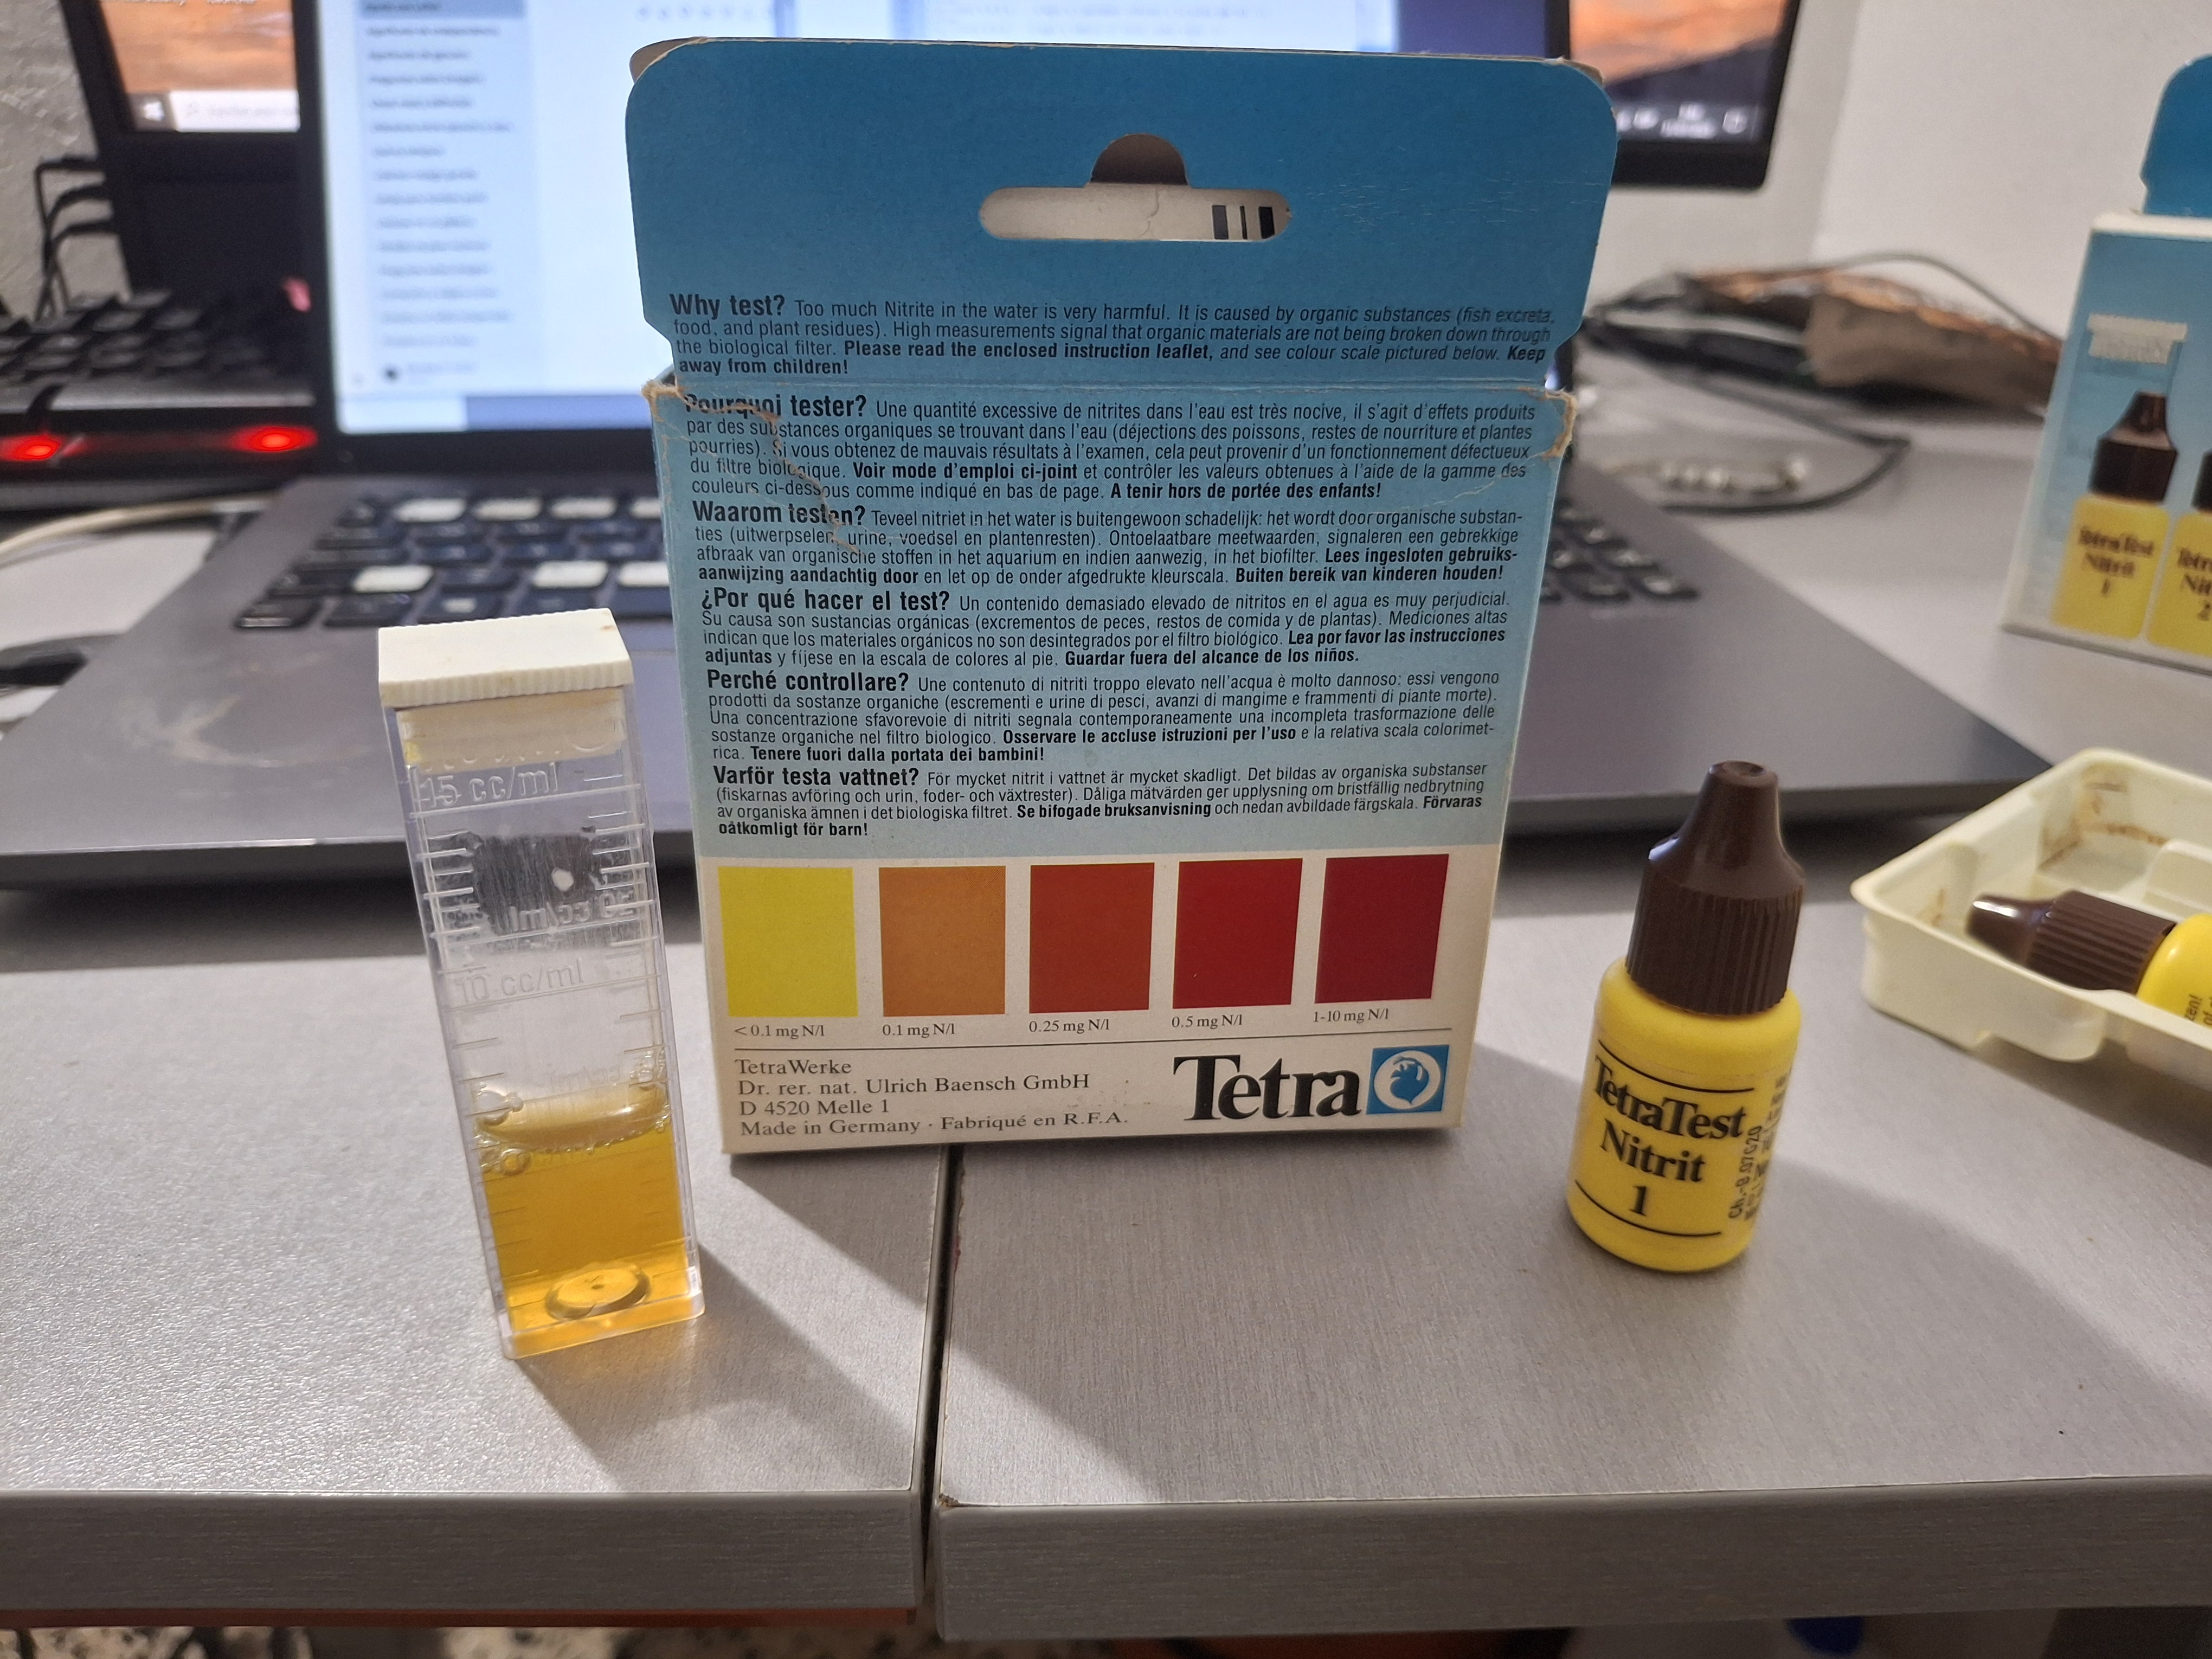
\includegraphics[width=0.5\textwidth]{./Figures/Tetra1.png}
\caption{TetraTest a la mostra numero 1}
\label{fig:TetraTestdeNitrit1}
\end{figure}

Com es pot observar a la figura~\ref{fig:TetraTestdeNitrit1}, segons el resultat del TetraTest, la concentració de nitrits és de 0,1 mg/L. Aquest resultat reforça, una vegada més, la meva hipòtesi que les tires reactives no són del tot fiables i que no es pot confiar plenament en els valors que indiquen.

Aquí finalitza el meu primer experiment. Els resultat han aportat més preguntes que respostes. A més a més dels resultats, espero que en els propers resultats tot sigui més fàcil des del punt de vista metodològic, és a dir, que el procediment ja es conegut i, per tant serà més rápid i eficient. També espero que els resultats obtinguts amb les tires convergeixin als valors oficials. En cas contrari, caldrà estudiar quins són les possibles causes d'aquestes diferències.
% Així va ser el meu primer experiment. No puc dir que n’hagi sortit del tot satisfet, ja que he tingut força decepcions, però també algunes alegries. Com que era el primer cop que ho feia, he après dels meus errors, ara sé què he de fer i què no la pròxima vegada, i tot plegat m’ha ajudat a organitzar-me molt millor. Una cosa és imaginar com serà tot i una altra molt diferent és viure-ho. Es podria dir que ha estat com una clatellada de realitat. Però, en el fons, aquesta és la gràcia de l’experimentació.


\clearpage

\section{Segon experiment}


Després d’obtenir alguns resultats sorprenents en el primer experiment, procedeixo fer un segon intent per confirmar si les diferències observades es tornen a repetir. En aquest cas, faig servir una nova mostra i mantinc les mateixes condicions que en l'experiment anterior per obtenir resultats fiables.

El material i el procediment que faig servir són els mateixos que en l’experiment anterior. L’únic canvi és la mostra: aquesta vegada no és d’aigua de casa meva, sinó que la vaig recollir en un bar d’un amic. Vaig escollir aquest lloc, i no casa seva o qualsevol altre, perquè volia fer una distinció clara entre l’aigua d’ús domèstic i la d’un establiment públic.
\begin{figure}[H]
\centering
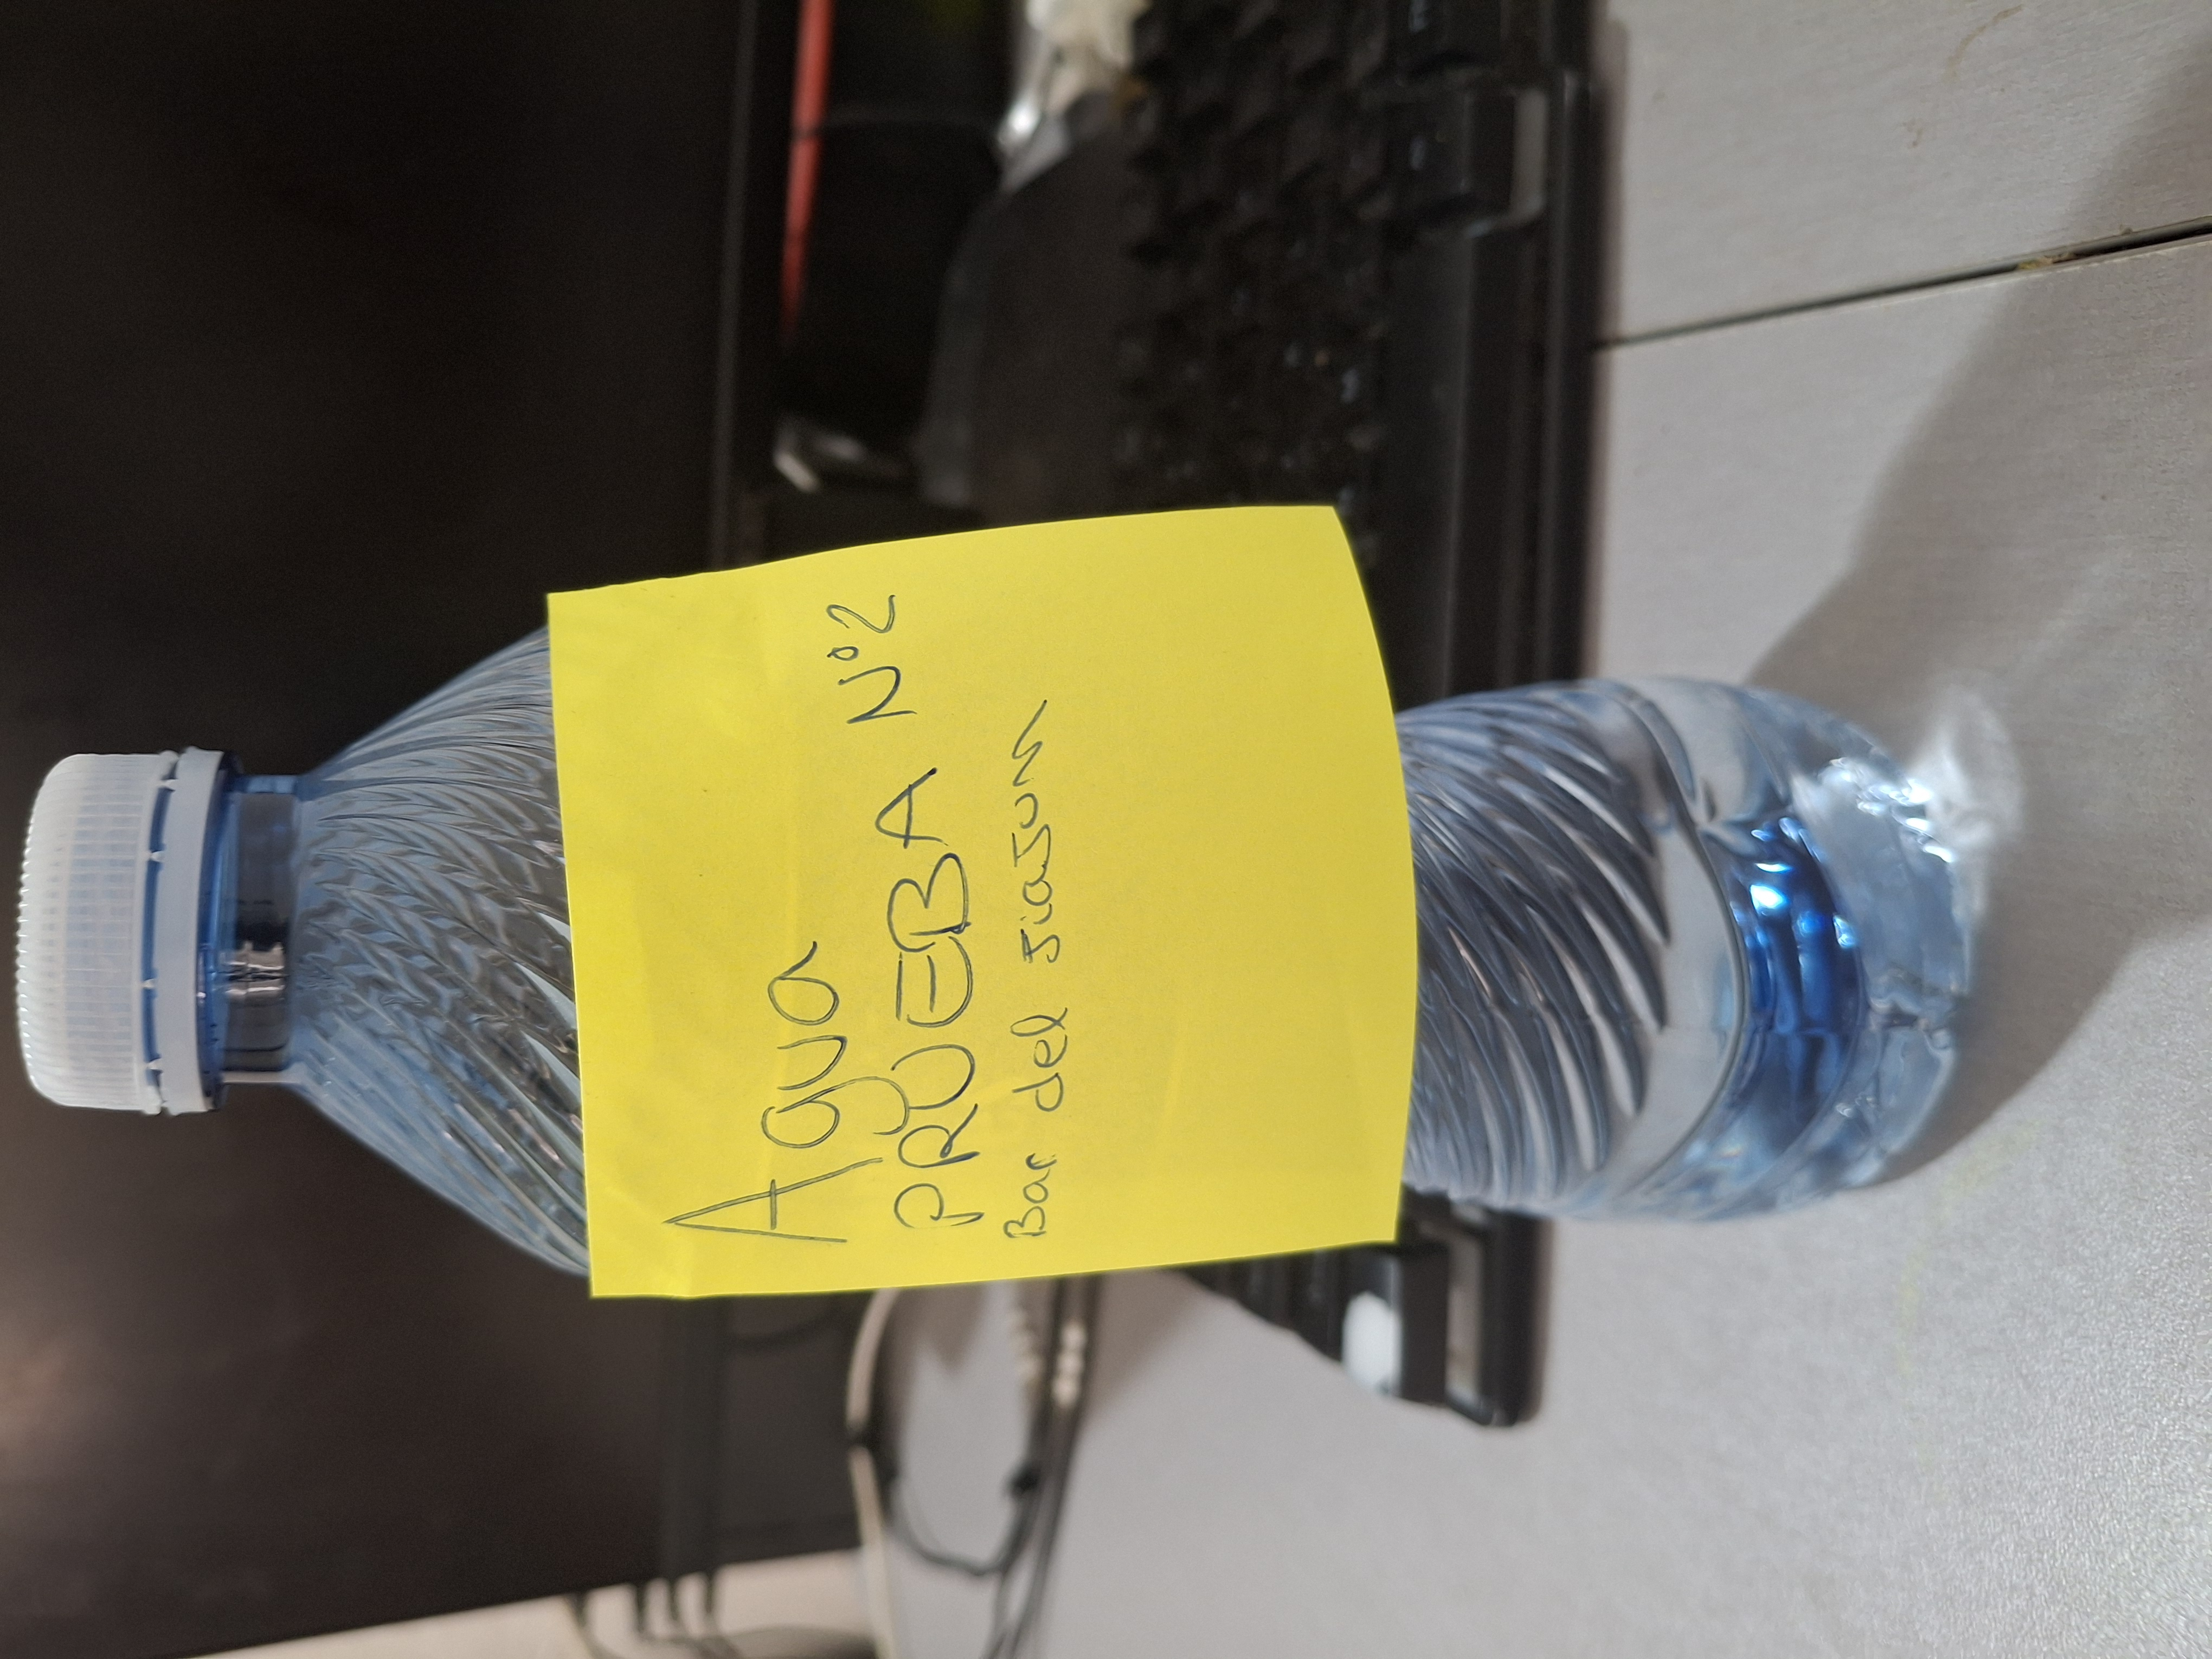
\includegraphics[width=0.45\textwidth, angle=270]{./Figures/AguaBar.png}
\caption{Aigua del bar}
\label{fig:AguaDelBar}
\end{figure}
Aquesta vegada volia extreure les dades d’una manera diferent. Tot i que la diferència en la metodologia no era gaire gran, volia experimentar amb una nova condició per veure si així els resultats de les tires reactives s’aproximaven més als valors originals.

L’única diferència respecte al primer experiment és que, en aquest cas, la tira sense exposició solar tampoc rebrà cap mena de llum: faré l’experiment completament a les fosques. En canvi, la tira amb exposició solar estarà sotmesa a una gran cuantitat de llum, utilitzant no només la llum del sol, sinó també la de diverses llanternes, amb l’objectiu d’aconseguir una diferència notable entre les dues tires reactives.

Després de fer totes les proves per extreure les dades, els resultats van ser els següents:
Es mostren els resultats obtinguts a la taula~\ref{tab:comparacio_dades2}.


\begin{table}[H]
\centering
\resizebox{\textwidth}{!}{
\begin{tabular}{|c|c|p{4.4cm}|}
\hline
\textbf{Paràmetre} & \textbf{Resultats sense llum en mg/L} & \textbf{Resultats amb llum en mg/L} \\
\hline
pH    & 7.8      & 7.6 \\
\hline
Alcalinitat total(CaCO$_3$)    & 40    & 120 \\
\hline
Carbonat     & 0     & 80 \\
\hline
Duresa (GH)   & 200          & 425  \\
\hline
Àcid cianúric    & 0     & 0 \\
\hline
Coure    & 0.2       & 0.2\\
\hline
Mercuri    & 0      & 0 \\
\hline
Clor total     & 0     & 0\\
\hline
 Clor lliure    & 0      & 0 \\
\hline
Brom  & 0      & 0\\
\hline
 Nitrit    & 0       & 0\\
\hline
Nitrat (NO$_3^-$)    & 0        & 0 \\
\hline
Ferro    & 0      & 0 \\
\hline
 Crom (VI)   & 0      & 0  \\
\hline
Plom   & 0     & 0  \\
\hline
Fluorur (F$^-$)    & 0      & 0 \\
\hline
\end{tabular}%
}
\caption{Resultats del segon experiment}
\label{tab:comparacio_dades2}
\end{table}
\vspace*{-0.5truecm}
Com podem observar a la taula~\ref{tab:comparacio_dades2}, la majoria de paràmetres no es detecten en aquesta mostra d’aigua. Tot i això, els que sí que hi apareixen presenten una gran diferència entre les dues tires: la que ha estat exposada a la llum i la que no.

Els valors que indiquen són força diferents (excepte en els casos dels paràmetres que no són presents a l’aigua). Tots, excepte del pH i el coure, mostren valors inferiors a la tira que no ha estat exposada a cap llum. Pel que fa al pH, sí que hi ha una petita reducció en la mostra amb exposició lumínica.

Aquestes diferències en els resultats feia especialment interessant la comparativa amb les dades oficials, ja que així podria determinar quin dels dos mètodes és el més adequat. Tal com vam veure en l’experiment anterior, les tires reactives no indiquen amb precisió la concentració de cada paràmetre, per això trobar mètodes alternatius més precisos és una nova via interessant per incorporar en el procés d’experimentació.

Després de consultar les dades oficials al portal d’Aigües de Barcelona~\cite{qualitatAigua}, vaig poder extreure les conclusions següents:

% Les taules es poden veure al \textit{Appendix}~\ref{s:A1}~ ~\nameref{tab:comparacio_aigua_sense_llum} i~\nameref{tab:comparacio_aigua_amb_llum}.\\

\vspace*{2truecm}

\begin{table}[H]
\centering
\resizebox{\textwidth}{!}{%
\begin{tabular}{|l|c|c|c|p{6.4cm}|}
\hline
\textbf{Paràmetre} & \textbf{Valor } & \textbf{Valor oficial} & \textbf{Unitats} & \textbf{Comentari} \\
&  \textbf{experimental} & & & \\
\hline \hline
pH & 7.8 & 7,3-8.3 & unitats pH & Dins dels valors minim-màxim.. \\
\hline
Alcalinitat total & 40 & 65.3-217 & mg CaCO$_3$/L & Valor experimental probablement incorrecte. \\
\hline
Carbonats & 0 & --- & mg /L & Informació no proporcionada. \\
\hline
Duresa total & 200 & 75.3-424 & mg GH/L & Millor aproximació al valor real que l'anterior experiment; dins dels valors minim-màxim. \\
\hline
Nitrat & 0 & $<$1-10.2 & mg NO$_3^-$ /L & Dins dels valors oficial. \\
\hline
Nitrit & 0 & ---& mg /L & Informació no proporcionada. \\
\hline
Clor total & 0 & --- & mg/L & Valor típic \\
\hline
Clor lliure & 0 & --- & mg/L & Idèntic al total; valor típic. \\
\hline
Ferro & 0 & --- & mg/L & Adequat; no hauria de tenir. \\
\hline
Fluorur & 0 & $<$0,2 & mg F$^-$ /L & Coincideix amb el valor esperat. \\
\hline
Crom (VI) & 0 & --- & mg/L & No present. \\
\hline
Plom & 0 & --- & mg/L & No detectat; adequat. \\
\hline
Àcid cianúric & 0 & --- & mg/L & No rellevant; igual que en l'experiment anterior. \\
\hline
Coure & 0.2 & --- & mg/L & Informació no detectada en aquest cas. \\
\hline
Brom & 0 & --- & mg/L & No detectat en aquest cas. \\
\hline
Mercuri & 0 & --- & mg/L & No detectat; correcte. \\
\hline
\end{tabular}%
}
\caption{Comparació entre els valors experimentals i els oficials de l'aigua del bar (sense exposició a cap font de llum}
\label{tab:comparacio_aigua_sense_llum}
\end{table}

\clearpage

\begin{table}[H]
\centering
\resizebox{\textwidth}{!}{%
\begin{tabular}{|l|c|c|c|p{6.2cm}|}
\hline
\textbf{Paràmetre} & \textbf{Valor } & \textbf{Valor oficial} & \textbf{Unitats} & \textbf{Comentari} \\
&  \textbf{experimental} & & & \\
\hline \hline
pH & 7.6 & 7,3-8.3 & unitats pH & Dins dels valors minim-màxim; com l'anterior cas. \\
\hline
Alcalinitat total & 120 & 65.3-217 & mg CaCO$_3$/L & Valor experimental dins dels limits. \\
\hline
Carbonats & 80 & --- & mg /L & Informació no proporcionada. \\
\hline
Duresa total & 425 & 75.3-424 & mg GH/L & Millor aproximació al valor real que abans, però no està dins dels valors minim-màxim; pot ser un petit error de extracció de dades. \\
\hline
Nitrat & 0 & $<$1-10.2 & mg NO$_3^-$ /L & Dins dels valors oficial; com l'anterior cas. \\
\hline
Nitrit & 0 & ---& mg /L & Informació no proporcionada. \\
\hline
Clor total & 0 & --- & mg/L & Valor típic \\
\hline
Clor lliure   & 0 & --- & mg/L & Idèntic al total; valor típic. \\
\hline
Ferro & 0 & --- & mg/L & Adequat; no hauria de tenir. \\
\hline
Fluorur & 0 & $<$0,2 & mg F$^-$ /L & Coincideix amb el valor esperat; com l'anterior cas. \\
\hline
Crom (VI) & 0 & --- & mg/L & No present. \\
\hline
Plom & 0 & --- & mg/L & No detectat; adequat. \\
\hline
Àcid cianúric & 0 & --- & mg/L & No rellevant; igual que en l'experiment anterior. \\
\hline
Coure & 0.2 & --- & mg/L & Informació no detectada en aquest cas. \\
\hline
Brom & 0 & --- & mg/L & No detectat en aquest cas. \\
\hline
Mercuri & 0 & --- & mg/L & No detectat; correcte. \\
\hline
\end{tabular}%
}
\caption{Comparació entre els valors experimentals i els oficials de l'aigua del bar (amb exposició a gran quantitat de llum}
\label{tab:comparacio_aigua_amb_llum}
\end{table}

Tal com podeu veure a les taules~\ref{tab:comparacio_aigua_sense_llum} i~\ref{tab:comparacio_aigua_amb_llum}, la mesura del pH, que en l’experiment anterior no havia coincidit amb cap de les dues tires, en aquest cas es troba dins dels valors esperats. I no només això, sinó que també altres valors, com la duresa total, es van situar dins dels límits en totes dues tires. Per tant, segons aquesta comparació, puc concloure que és millor exposar la tira a la llum.
% A més, els valors que ens aporten són diferents, per tant, ens hem de limitar només als que coincideixen en ambdós casos.

És cert que molts paràmetres no els puc comparar per no tenir dades oficials, però, gràcies als que sí que disposo, puc inferir quins dels valors restants podrien ser fiables. Aquesta comparació ajuda a fer-se una idea general de la coherència dels resultats.

Un cop obtingudes les dades de les tires, em faltava verificar el pH amb el mesurador específic i utilitzar el TetraTest de nitrit per confirmar el valor de 0 mg/L indicat a les tires reactives.

El valor obtingut amb el mesurador de pH va ser de 7,3 mg/L. Això confirma que la mostra es troba dins dels límits recomanats segons les dades oficials.

Finalment, el TetraTest va donar un valor de 0,1 mg/L. Aquest resultat contradiu lleugerament les tires, que mostraven 0 mg/L. Tot i així, cal tenir en compte que una diferència tan petita pot no ser apreciable visualment en una tira reactiva, especialment si el canvi de color és poc tan apreciable. Per tant, podria tractar-se simplement d’un error causat per la incapacitat de distingir dos colors molts semblants a ull nu.

\bigskip


\textbf{Com a conclusió}, després de comparar una mostra d’aigua d’un domicili amb una d’un establiment públic, puc afirmar que la concentració de substàncies és força diferent en els dos casos. El tractament de l’aigua pot influir notablement en els valors detectats. A més, aquest segon experiment m’ha servit per reforçar la importància de fer més d’una prova i contrastar resultats mitjançant diferents mètodes.

Amb això, finalitzo el segon experiment. Tal com havia previst, ha estat més ràpid que el primer.%, i espero que el tercer i ùltim, ho sigui encara més.
% \vspace{10cm}
\clearpage

\section{Tercer experiment}

Finalment, el tercer i darrer experiment d’aquest treball de recerca vol ampliar l'estudi sobre l'efectivitat de les tires reactives depenent d'un nou paràmetre: el temps. A diferència del cas anterior, ara la llum no serà el factor a estudiar, ara valorarem si el temps en mesurar la reacció afecta als resultats.
%vegada, la meva idea era jugar amb el temps d’espera. Normalment, un vegada submergida la tira en l’aigua, cal deixar-la reposar uns 60 segons perquè els colors apareguin correctament. El que proposo ara és fer una comparació entre dues tires modificant aquest temps.

En el primer cas, no deixaré gaire temps a la tira per reaccionar: només 5 segons. Tal com he pogut observar en les proves anteriors, a partir de 2 segons la tira ja comença a mostrar els seus colors, per això vull analitzar què passa si gairebé no li dono temps. Òbviament, sé que el temps que trigo a mirar i comparar els colors també influeix, així que, a més de fer-ho tan ràpid com pugui un cop passats els 5 segons, faré una foto de la tira als cinc segons per poder corroborar els resultats.

En canvi, en el segon cas, deixaré que la tira s’assequi durant 2 minuts, és a dir, 120 segons, el doble del temps recomanat habitualment.

Els passos a seguir seran exactament els mateixos que en els experiments anteriors. L’única diferència serà la mostra d’aigua. Aquesta vegada vaig anar a casa d’un amic per recollir una mostra de l’aigua de casa seva, que vaig emmagatzemar en una ampolla de plàstic degudament etiquetada.

\begin{figure}[H]
\centering
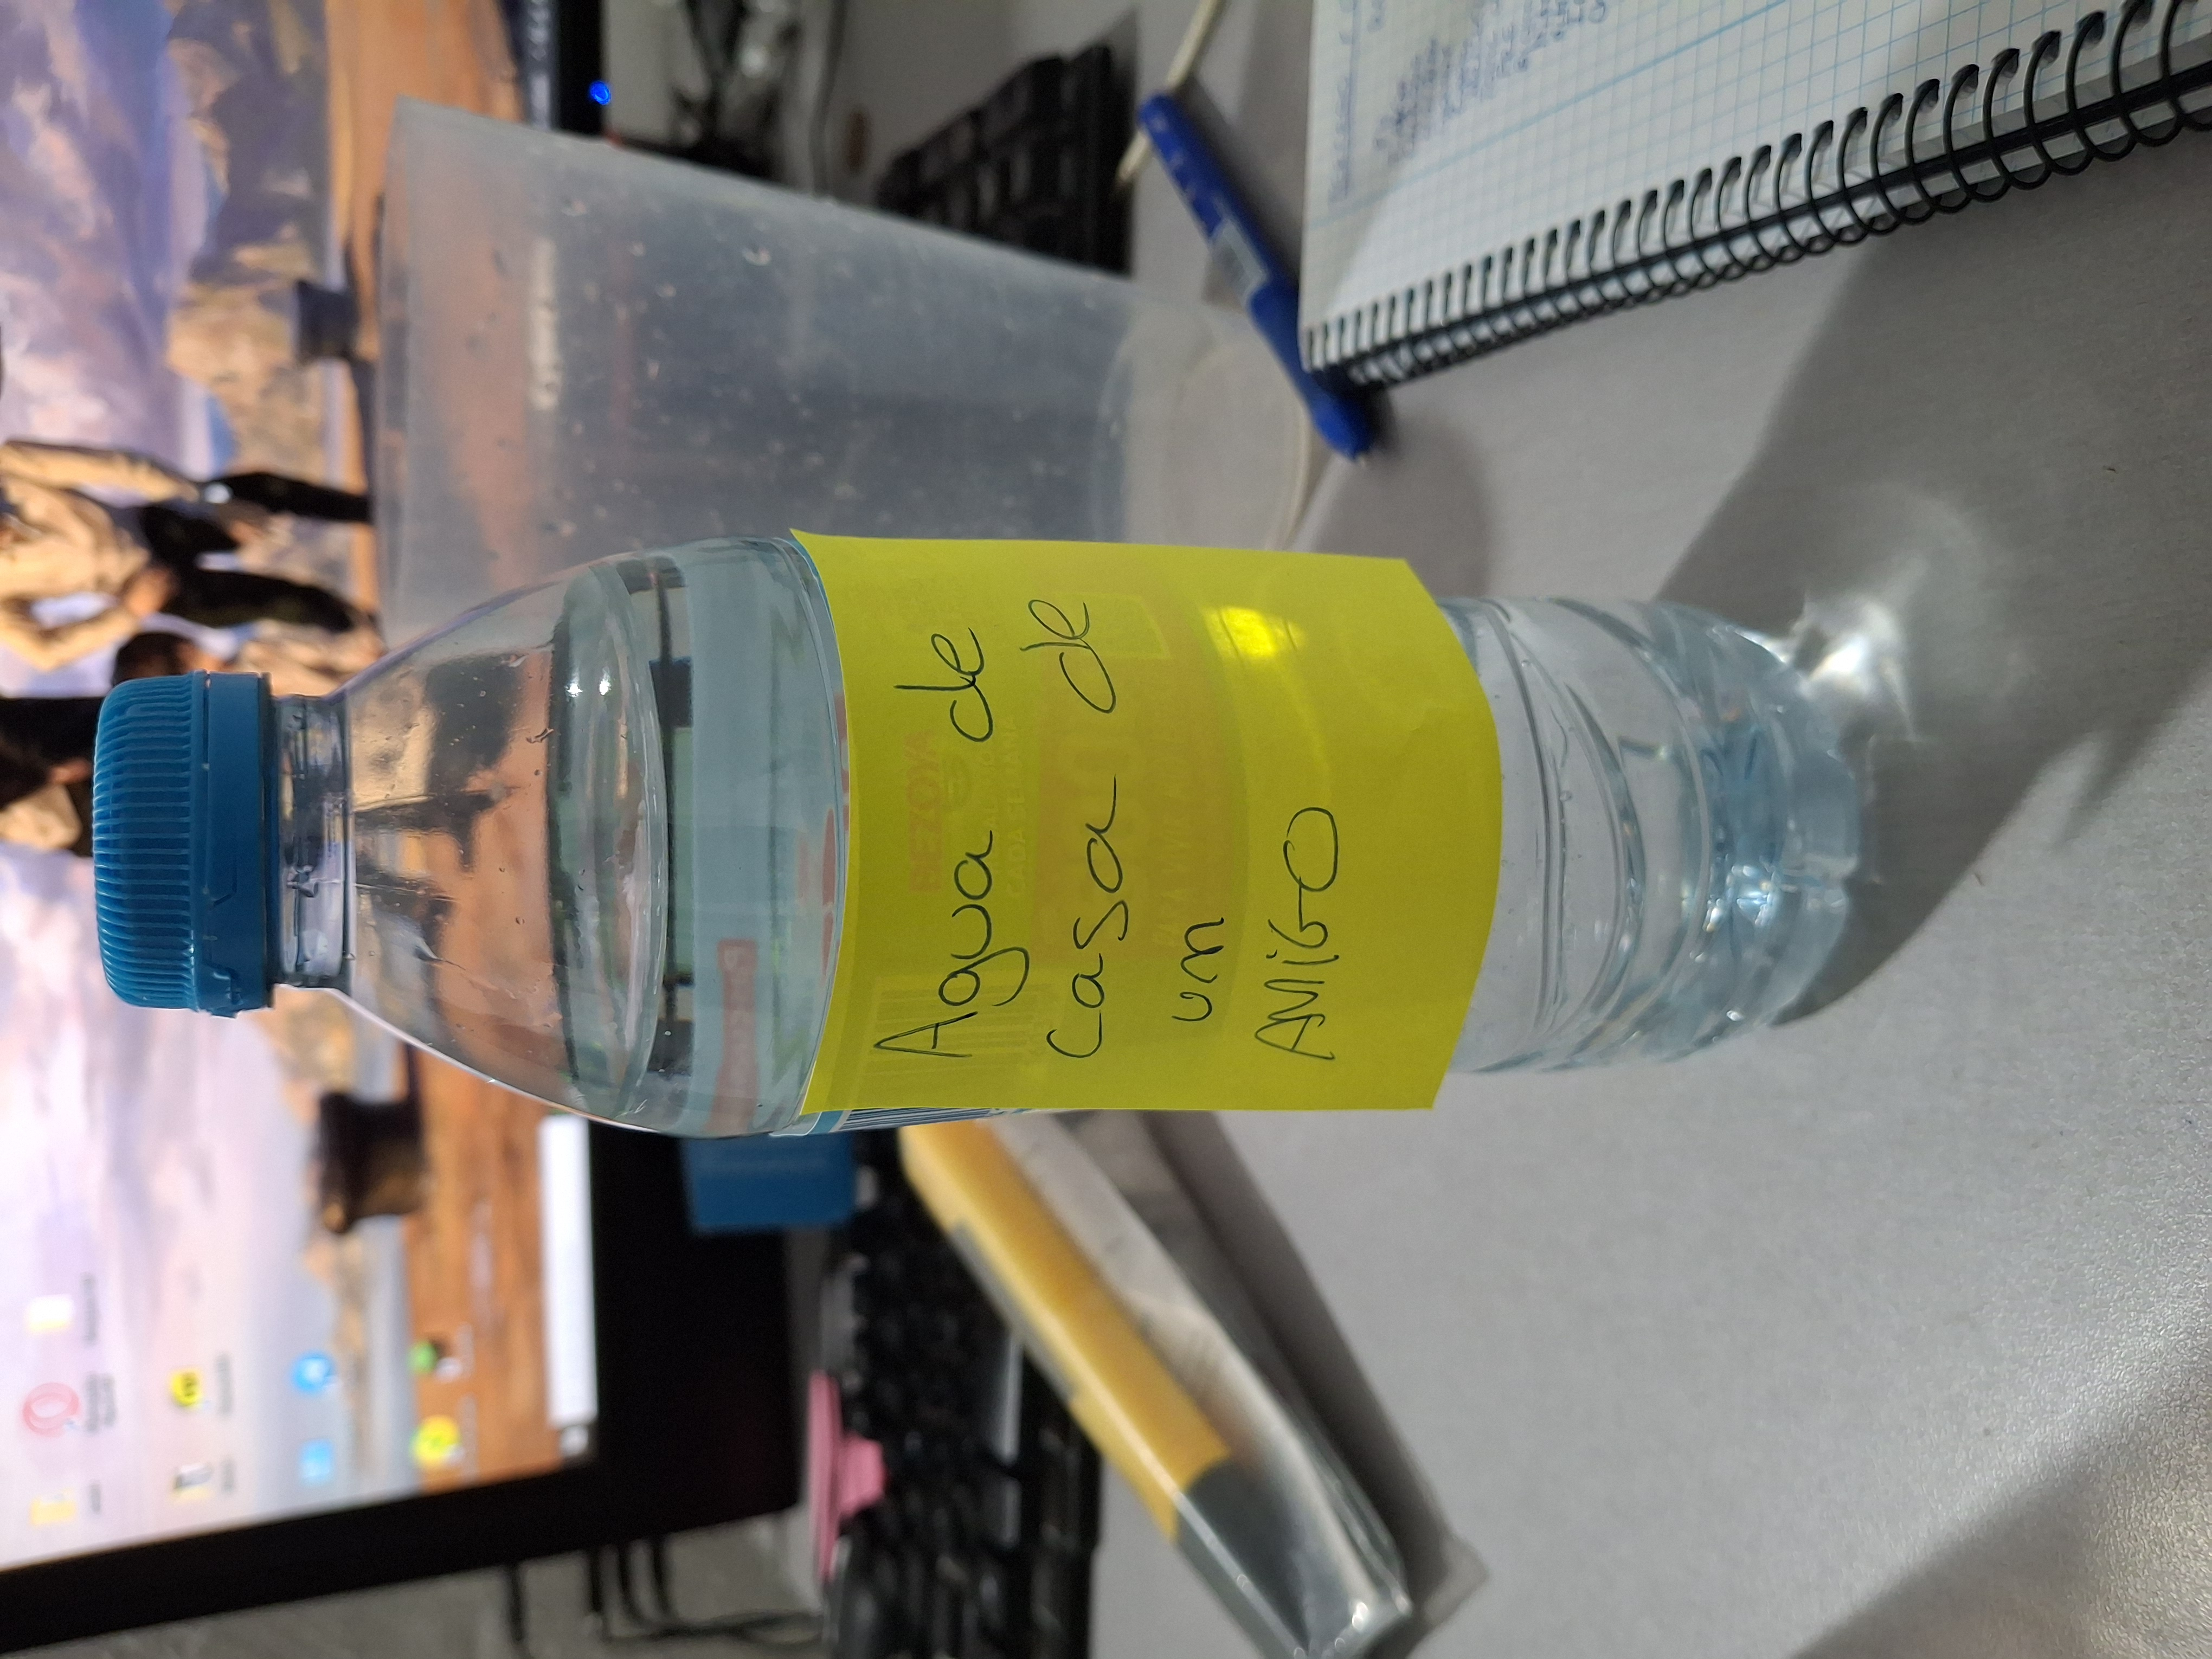
\includegraphics[width=0.5\textwidth, angle=270]{./Figures/ex3.png}
\caption{Mostra número 3}
\label{fig:Mostra3}
\end{figure}
\clearpage
Els resultats obtinguts es mostren a la taula~\ref{tab:comparacio_dades_3}.
% Després de fer les proves amb les tires reactives, aquests en van ser els resultats:
%
% Es mostren els resultats obtinguts al \textit{Appendix}~\ref{s:A1}, a la taula ~\nameref{tab:comparacio_dades_3}.

\vspace*{2truecm}
\begin{table}[H]
\centering
\resizebox{\textwidth}{!}{%
\begin{tabular}{|l|c|c|c|p{5.2cm}|}
\hline
\textbf{Paràmetre} & \textbf{Tira } & \textbf{Tira } & \textbf{Unitats} & \textbf{Comentari} \\
& \textbf{(5 segons)} & \textbf{(120 segons)} & &  \\
\hline \hline
pH & 8.4 & 8.4 & unitats pH & No hi ha difèrencia en cap cas. \\
\hline
Alcalinitat total & 180 & 240 & mg CaCO$_3$/L & Difèrencia bastant elevada. \\
\hline
Carbonats & 180 & 240 & mg/L & Difèrencia bastant elevada. \\
\hline
Duresa total & 335 & 425 & mg GH/L & Difèrencia bastant elevada. . \\
\hline
Nitrat & 10 & 25 & mg NO$_3^-$ /L & Difèrencia bastant elevada. \\
\hline
Nitrit & 0 & 0 & mg /L & Cap difèrencia. \\
\hline
Clor total & 0 & 0 & mg/L & Cap difèrencia. \\
\hline
Clor lliure & 0 & 0 & mg/L & Cap difèrencia. \\
\hline
Ferro & 0 & 0 & mg/L & Cap difèrencia. \\
\hline
Fluorur & 0 & 0 & mg F$^-$ /L & Cap difèrencia. \\
\hline
Crom (VI) & 0 & 0 & mg/L & Cap difèrencia. \\
\hline
Plom & 0 & 0 & mg/L & Cap difèrencia. \\
\hline
Àcid cianúric & 0 & 0 & mg/L & Cap difèrencia. \\
\hline
Coure & 0.2 & 0.5 & mg/L & Difèrencia de 0,3 mg/L. \\
\hline
Brom & 0 & 0 & mg/L & Cap difèrencia. \\
\hline
Mercuri & 0 & 0 & mg/L & Cap difèrencia.. \\
\hline
\end{tabular}%
}
\caption{Comparació entre els valors experimentals al tercer experiment}
\label{tab:comparacio_dades_3}
\end{table}

\vspace*{1truecm}
Un cop finalitzada l’extracció de dades amb les tires reactives, el següent pas va ser comparar els resultats obtinguts amb els valors oficials disponibles tal i com mostren les taules~\ref{tab:comparacio_aigua_5s} i~\ref{tab:comparacio_aigua_120s}

\clearpage

\begin{table}[H]
\centering
\resizebox{\textwidth}{!}{%
\begin{tabular}{|l|c|c|c|p{4.2cm}|}
\hline
\textbf{Paràmetre} & \textbf{Valor experimental} & \textbf{Valor oficial} & \textbf{Unitats} & \textbf{Comentari} \\
\hline \hline
pH & 8.4 & 7,3-8.3 & unitats pH & Supera per poc al valor màxim. \\
\hline
Alcalinitat total & 180 & 65.3-217 & mg CaCO$_3$/L & Valor experimental dins dels limits. \\
\hline
Carbonats & 180 & --- & mg /L & Informació no proporcionada. \\
\hline
Duresa total & 335 & 75.3-424 & mg GH/L & Valor experimental dins dels limits. \\
\hline
Nitrat & 10 & $<$1-10.2 & mg NO$_3^-$ /L & Valor experimental dins dels limits. \\
\hline
Nitrit & 0 & ---& mg /L & Informació no proporcionada. \\
\hline
Clor total & 0 & --- & mg/L & Valor típic \\
\hline
Clor lliure & 0 & --- & mg/L & Idèntic al total; valor típic. \\
\hline
Ferro & 0 & --- & mg/L & Adequat; no hauria de tenir. \\
\hline
Fluorur & 0 & $<$0,2 & mg F$^-$ /L & Coincideix amb el valor esperat. \\
\hline
Crom (VI) & 0 & --- & mg/L & No present. \\
\hline
Plom & 0 & --- & mg/L & No detectat; adequat. \\
\hline
Àcid cianúric & 0 & --- & mg/L & No rellevant; igual que en els experiments anteriors. \\
\hline
Coure & 0.2 & --- & mg/L & Informació no detectada en aquest cas. \\
\hline
Brom & 0 & --- & mg/L & No detectat en aquest cas. \\
\hline
Mercuri & 0 & --- & mg/L & No detectat; correcte. \\
\hline
\end{tabular}%
}
\caption{Comparació entre els valors experimentals i els oficials, tira anb durada 5 segons}
\label{tab:comparacio_aigua_5s}
\end{table}

\begin{table}[H]
\centering
\resizebox{\textwidth}{!}{%
\begin{tabular}{|l|c|c|c|p{4.2cm}|}
\hline
\textbf{Paràmetre} & \textbf{Valor experimental} & \textbf{Valor oficial} & \textbf{Unitats} & \textbf{Comentari} \\
\hline \hline
pH & 8.4 & 7,3-8.3 & unitats pH & Supera per poc al valor màxim; com abans. \\
\hline
Alcalinitat total & 240 & 65.3-217 & mg CaCO$_3$/L & Valor experimental lluny dels limits. \\
\hline
Carbonats & 240 & --- & mg /L & Informació no proporcionada. \\
\hline
Duresa total & 425 & 75.3-424 & mg GH/L & Valor experimental fora dels limits per 1 mg/L; ppot ser un error visual de part meva. \\
\hline
Nitrat & 25 & $<$1-10.2 & mg NO$_3^-$ /L & Valor experimental lluny dels limits. \\
\hline
Nitrit & 0 & ---& mg /L & Informació no proporcionada. \\
\hline
Clor total & 0 & --- & mg/L & Valor típic \\
\hline
Clor lliure & 0 & --- & mg/L & Idèntic al total; valor típic. \\
\hline
Ferro & 0 & --- & mg/L & Adequat; no hauria de tenir. \\
\hline
Fluorur & 0 & $<$0,2 & mg F$^-$ /L & Coincideix amb el valor esperat. \\
\hline
Crom (VI) & 0 & --- & mg/L & No present. \\
\hline
Plom & 0 & --- & mg/L & No detectat; adequat. \\
\hline
Àcid cianúric & 0 & --- & mg/L & No rellevant; igual que en els experiments anteriors. \\
\hline
Coure & 0.5 & --- & mg/L & Informació no detectada en aquest cas. \\
\hline
Brom & 0 & --- & mg/L & No detectat en aquest cas. \\
\hline
Mercuri & 0 & --- & mg/L & No detectat; correcte. \\
\hline
\end{tabular}%
}
\caption{Comparació entre els valors experimentals i els oficials, tira anb durada 120 segons}
\label{tab:comparacio_aigua_120s}
\end{table}

Amb aquests resultats i la comparativa realitzada, he arribat a la conclusió que la tira amb una durada de només 5 segons proporciona valors més propers als valors oficials. Per tant, aquesta opció sembla ser més fiable que deixar assecar la tira durant 120 segons.

Un cop arribat aquesta conclusió sobre les tires reactives, només em quedava completar el procés amb dues últimes mesures: determinar el pH amb el mesurador de pH i verificar el valor del nitrit amb el TetraTest de nitrit.
\begin{table}[H]
\centering
\begin{tabular}{|c|c|}
\hline
Paràmetre/instrument & Valor en mg/L \\
\hline
Mesurador de pH    & 7.4  \\
\hline
TetraTest de nitrit    & 0.1  \\
\hline
\end{tabular}%
\caption{Valors experimentals amb mesurador de pH i TetraTest de nitrit}
\label{tab:valors_tetra_pH}
\end{table}

Com es pot observar a la taula~ \ref{tab:valors_tetra_pH}, el valor del pH mesurat amb el mesurador es troba dins dels límits establerts, a diferència del que indiquen les tires reactives. Pel que fa al TetraTest de nitrit, com en els casos anteriors, el resultat ha estat de 0,1 mg/L.

La meva hipòtesi és que el valor real del nitrit és, efectivament, 0,1 mg/L, però que aquesta petita variació no és suficient per provocar un canvi en el color de les tires reactives, i per això aquestes mostren un valor de 0 mg/L.

% Aquí finalitza la meva part pràctica. He anat força ràpid amb l’últim experiment. Tot i això, ha estat un experiment més complicat del que m’imaginava al principi. Sincerament, no he quedat del tot satisfet amb el resultat. Tenia expectatives més altes, però, malauradament, el fet de no poder trobar dades oficials de molts dels paràmetres ha afectat negativament la meva motivació.

% Tot i així, amb els paràmetres dels quals sí que disposava de valors oficials, he pogut extreure conclusions clares i estic satisfet amb els resultats obtinguts. Han estat útils per reforçar les meves hipòtesis i entendre millor el funcionament de les tires reactives i la qualitat de l’aigua segons la seva procedència.

Aquí finalitza la meva part pràctica en la que no nomès he pogut reproduir els resultats que ofereix Aigües de Barcelona, sinó que he pogut estudiar un parell de paràmetres que poden millorar la fiabilitat de les tires reactives.

\section{Resultats de la part pràctica} \label{s:resultats}
Després de realitzar els tres experiments amb diferents mostres d’aigua i condicions de mesura, puc afirmar que l’ús de tires reactives presenta certes limitacions, però també ofereix informació rellevant quan es fa servir correctament.

En el primer experiment vaig comprovar que les tires, tot i donar una idea aproximada dels valors, no sempre coincidien amb les dades oficials. Això em va portar a pensar que factors externs podien influir en els resultats. En el segon experiment, introduint la variable de la llum, vaig poder veure que l’exposició a la llum millorava notablement la coincidència amb els valors oficials, especialment pel que fa a la duresa i l’alcalinitat. Finalment, en el tercer experiment vaig analitzar l’efecte del temps d’espera, i vaig observar que un temps massa llarg provocava desviacions considerables en diversos paràmetres, mentre que una lectura ràpida (als 5 segons) era més fidel a les dades reals.

Amb tot això, puc concloure que les tires reactives poden ser una eina útil per a una primera aproximació de la qualitat de l’aigua, però cal tenir en compte certes condicions per tal que els resultats siguin més fiables. A més, comparar els valors amb altres mètodes (mesurador de pH i TetraTest) m’ha permès validar que algunes diferències no són degudes a errors de la mostra, sinó a la pròpia limitació visual i tècnica de les tires.

A partir d’aquests experiments, he elaborat una guia pràctica perquè altres usuaris puguin utilitzar les tires d’una manera més correcta i treure’n conclusions més ajustades a la realitat.

\subsection{Guia per utilitzar tires reactives}

Com a usuari de les tires he trobat informacions contradictòries sobre el seu ús, i per descomptat, cap d'elles en català. Per tant, a continuació trobareu un manual per a fer servir aquest material i obtenir resultats tan fiables com sigui possible.

\begin{enumerate}
    \item \textbf{Preparació de la mostra} \\
    Recollir l’aigua en un recipient net i preferiblement de plàstic o vidre. Evitar l’exposició a contaminants externs abans de fer la prova.

    \item \textbf{Temps d’espera} \\
    El temps recomanat pels fabricants sol ser d’uns 60 segons, però segons les meves proves, una lectura ràpida als \textbf{5-10 segons} pot oferir valors més propers als reals en alguns paràmetres sensibles (com nitrats i alcalinitat). Evitar temps massa llargs (més de 120 segons), ja que els resultats tendeixen a desviar-se.

    \item \textbf{Condicions de llum} \\
    La llum és un factor important. És recomanable fer la lectura en un lloc ben il·luminat, i fins i tot reforçar amb llum artificial si cal. Evitar llegir les tires en condicions de foscor o amb poca llum, ja que això pot fer perdre matisos en els colors.

    \item \textbf{Comparació de colors} \\
    Comparar immediatament els colors amb l’escala de la tira, però si hi ha dubtes, fer una fotografia de la tira per revisar-la amb més calma. Cal tenir en compte que algunes diferències mínimes poden ser difícils de distingir a simple vista.

    \item \textbf{Contrast amb altres mètodes} \\
    Sempre que sigui possible, contrastar els resultats de les tires amb altres instruments (mesuradors de pH, TetraTest, etc.). Això ajuda a validar la fiabilitat i a descartar possibles errors visuals.

    \item \textbf{Interpretació dels resultats} \\
    Les tires reactives són útils com a \textbf{indicador general}, però no substitueixen les dades oficials ni els mètodes de laboratori. S’han d’interpretar com una aproximació, especialment en els paràmetres que no mostren una correspondència directa amb les dades oficials.
\end{enumerate}

Per tal de validar aquesta guia i comprovar que les recomanacions proposades realment funcionen, he dut a terme un total de cinc experiments amb diferents mostres d’aigua i condicions diverses. Els resultats obtinguts en aquests experiments, que es poden consultar detalladament a l'\textit{Apèndix}~\ref{a:guia}. Així doncs, la guia no només té una base teòrica, sinó també experimental, i ofereix un recurs pràctic per a futurs usuaris.



